% LaTeX Template For MATH 490 @ VCU
\documentclass[11pt]{article}

\usepackage{hyperref}
\usepackage{amsmath}
\usepackage{amsthm}
\usepackage{amssymb}
\usepackage{enumerate}
\usepackage{enumitem}
\usepackage{titlesec}
\usepackage{multicol}
\usepackage{multirow}
\usepackage{mathtools}
\usepackage{mdframed}
\usepackage{tocloft}
\usepackage{tcolorbox}
\usepackage{extarrows}

\setlist{nosep}
% \setlist[enumerate]{label=(\alph*)}

\renewcommand{\arraystretch}{0.85}

\definecolor{defcolor}{RGB}{255,236,236}    % light red
\definecolor{ngtcolor}{RGB}{255,242,242}    % lighter red
\definecolor{lnkcolor}{RGB}{0,0,180}        % blue
\definecolor{thmcolor}{RGB}{236,236,255}    % light blue
\definecolor{lemcolor}{RGB}{239,239,255}    % lighter blue
\definecolor{procolor}{RGB}{242,242,255}    % lighter lighter blue
\definecolor{crlcolor}{RGB}{245,245,255}    % lighter lighter lighter blue
\definecolor{xmpcolor}{RGB}{255,240,225}    % light orange
\definecolor{rmkcolor}{RGB}{233,255,235}    % light green
\definecolor{axicolor}{RGB}{255,255,233}    % light yellow
\definecolor{notcolor}{RGB}{255,255,244}    % lighter yellow
\definecolor{whacolor}{RGB}{250,250,250}    % lighter gray
\definecolor{reccolor}{RGB}{255,244,255}    % lighter purple

\hypersetup{
    colorlinks,
    citecolor=lnkcolor,
    filecolor=lnkcolor,
    linkcolor=lnkcolor,
    urlcolor=lnkcolor
}

\newtheoremstyle{break}
    {\topsep/1.5} % space above
    {\topsep/2.2} % space below
    {}          % body font
    {}          % indent amount
    {\rmfamily} % theorem head font
    {.}          % punctuation after theorem head
    {0.5em}  % space after theorem head
    {\textbf{\thmname{#1}\thmnumber{ #2}}\thmnote{\text{ (#3)}}}
                % theorem hed spec. (empty = "normal")

\newtheoremstyle{no_label}
    {\topsep/1.5} % space above
    {\topsep/2.2} % space below
    {}          % body font
    {}          % indent amount
    {\rmfamily} % theorem head font
    {.}          % punctuation after theorem head
    {0.5em}  % space after theorem head
    {\textbf{\thmname{#1}\thmnumber{}}\thmnote{\text{ (#3)}}}
                % theorem hed spec. (empty = "normal")

\theoremstyle{break}
\newmdtheoremenv[
    backgroundcolor=thmcolor,
    linecolor=black,
    linewidth=1pt,
    topline=true,
    bottomline=true,
    rightline=true,
    skipabove=\topsep/1.5,
    skipbelow=\topsep/2.2
]{theorem}{Theorem}[section]
\newmdtheoremenv[
    backgroundcolor=crlcolor,
    linecolor=black,
    linewidth=1pt,
    topline=true,
    bottomline=true,
    rightline=true,
    skipabove=\topsep/1.5,
    skipbelow=\topsep/2.2
]{corollary}[theorem]{Corollary}
\newmdtheoremenv[
    backgroundcolor=lemcolor,
    linecolor=black,
    linewidth=1pt,
    topline=true,
    bottomline=true,
    rightline=true,
    skipabove=\topsep/1.5,
    skipbelow=\topsep/2.2
]{lemma}[theorem]{Lemma}
\newmdtheoremenv[
    backgroundcolor=axicolor,
    linecolor=black,
    linewidth=1pt,
    topline=true,
    bottomline=true,
    rightline=true,
    skipabove=\topsep/1.5,
    skipbelow=\topsep/2.2
]{axiom}[theorem]{Axiom}
\newmdtheoremenv[
    backgroundcolor=procolor,
    linecolor=black,
    linewidth=1pt,
    topline=true,
    bottomline=true,
    rightline=true,
    skipabove=\topsep/1.5,
    skipbelow=\topsep/2.2
]{proposition}[theorem]{Proposition}
\newmdtheoremenv[
    backgroundcolor=defcolor,
    linecolor=black,
    linewidth=1pt,
    topline=true,
    bottomline=true,
    rightline=true,
    skipabove=\topsep/1.5,
    skipbelow=\topsep/2.2
]{definition}[theorem]{Definition}
\newmdtheoremenv[
    backgroundcolor=rmkcolor,
    linecolor=black,
    linewidth=1pt,
    topline=true,
    bottomline=true,
    rightline=true,
    skipabove=\topsep/1.5,
    skipbelow=\topsep/2.2
]{remark}[theorem]{Remark}
\newmdtheoremenv[
    backgroundcolor=xmpcolor,
    linecolor=black,
    linewidth=1pt,
    topline=true,
    bottomline=true,
    rightline=true,
    skipabove=\topsep/1.5,
    skipbelow=\topsep/2.2
]{example}[theorem]{Example}
\newmdtheoremenv[
    backgroundcolor=whacolor,
    linecolor=black,
    linewidth=1pt,
    topline=true,
    bottomline=true,
    rightline=true,
    skipabove=\topsep/1.5,
    skipbelow=\topsep/2.2
]{problem}[theorem]{Problem}
\newmdtheoremenv[
    backgroundcolor=whacolor,
    linecolor=black,
    linewidth=1pt,
    topline=true,
    bottomline=true,
    rightline=true,
    skipabove=\topsep/1.5,
    skipbelow=\topsep/2.2
]{exercise}[theorem]{Exercise}

\theoremstyle{no_label}
\newmdtheoremenv[
    backgroundcolor=whacolor,
    linecolor=black,
    linewidth=1pt,
    topline=true,
    bottomline=true,
    rightline=true,
    skipabove=\topsep/1.5,
    skipbelow=\topsep/2.2
]{question}{Question}
\newmdtheoremenv[
    backgroundcolor=reccolor,
    linecolor=black,
    linewidth=1pt,
    topline=true,
    bottomline=true,
    rightline=true,
    skipabove=\topsep/1.5,
    skipbelow=\topsep/2.2
]{recall}{Recall}
\newmdtheoremenv[
    backgroundcolor=notcolor,
    linecolor=black,
    linewidth=1pt,
    topline=true,
    bottomline=true,
    rightline=true,
    skipabove=\topsep/1.5,
    skipbelow=\topsep/2.2
]{notation}{Notation}

\DeclareMathOperator{\arcsec}{arcsec}
\DeclareMathOperator{\arccot}{arccot}
\DeclareMathOperator{\arccsc}{arccsc}
\DeclareMathOperator{\interior}{int}
\DeclareMathOperator{\closure}{cl}
\DeclareMathOperator{\boundary}{bd}

\newcommand{\derivative}{D\!\,}
\newcommand{\scndderivative}{D^2\!\,}
\newcommand{\dirderivative}[1]{D_{#1}\:}
\newcommand{\pderivative}[2]{\dfrac{\partial {#1}}{\partial {#2}}}
\newcommand{\scndpderivative}[3]{\dfrac{\partial^2 {#1}}{\partial {#3}\partial {#2}}}
\newcommand{\dd}{\text{d}}
\newcommand{\ddi}{\text{$\,$d}}
\newcommand{\qqed}{{\hfill$\blacksquare$}}
\newcommand{\defeq}{\overset{\text{def}}{=}}
\newcommand{\transpose}{\text{T}}
\newcommand{\bbR}{\mathbb{R}}
\newcommand{\bbN}{\mathbb{N}}
\newcommand{\calL}{\mathcal{L}}
\newcommand{\bfa}{\textbf{a}}
\newcommand{\bfb}{\textbf{b}}
\newcommand{\bfe}{\textbf{e}}
\newcommand{\bff}{\textbf{f}}
\newcommand{\bfg}{\textbf{g}}
\newcommand{\bfh}{\textbf{h}}
\newcommand{\bfr}{\textbf{r}}
\newcommand{\bfv}{\textbf{v}}
\newcommand{\bfu}{\textbf{u}}
\newcommand{\bfx}{\textbf{x}}
\newcommand{\bfy}{\textbf{y}}
\newcommand{\pfexercise}{This is an exercise left to the reader.}

\linespread{2}
\setlength{\textwidth}{6.9in}
\setlength{\textheight}{9.2in}
\setlength{\oddsidemargin}{-0.2in}
\setlength{\evensidemargin}{-0.2in}
\setlength{\topmargin}{-0.2in}
\setlength{\headheight}{0in}
\setlength{\headsep}{0in}
\setlength{\footskip}{0.5in}
\setlength{\multicolsep}{6.2pt}
\setlength{\delimitershortfall}{13pt}
\delimiterfactor=100

\setcounter{section}{0}
\numberwithin{equation}{theorem}

\makeatletter
\newcommand{\vast}{\bBigg@{4}}
\newcommand{\Vast}{\bBigg@{5}}
\makeatother

\newcommand*\samethanks[1][\value{footnote}]{\footnotemark[#1]}

\title{\textbf{Introduction to Linear Algebra}}
\author{Chang, Yung-Hsuan}

\begin{document}
\maketitle
\thispagestyle{empty}
\newpage
\pagenumbering{roman}
\newpage
\phantomsection
\addcontentsline{toc}{section}{Contents}
\tableofcontents
\newpage

\phantomsection
\addcontentsline{toc}{section}{Preface}
\section*{Preface}

This note is summarized by Yung-Hsuan Chang as he took the course MIT 18.16 Linear Algebra instructed by Gilbert Strang.

\newpage
\pagenumbering{arabic}

\section{System of Linear Equations}

The fundamental problem of linear algebra is to solve $n$ linear equations in $n$ unknowns. For example, the case when $n=2$,
\begin{equation}\label{example equation for the essense of linear algebra}
    \left\{\begin{array}{rl}
        2x-y\!\!\!&=0;\\
        -x+2y\!\!\!&=3.
    \end{array}\right.
\end{equation}
There are three main ways to see this problem:
\begin{enumerate}
    \item row picture,
    \item column picture, and
    \item matrix picture.
\end{enumerate}

Row picture describes the relationship among equations. Take (\ref{example equation for the essense of linear algebra}) for an example, the graph shows the concept of row picture.

\begin{center}
    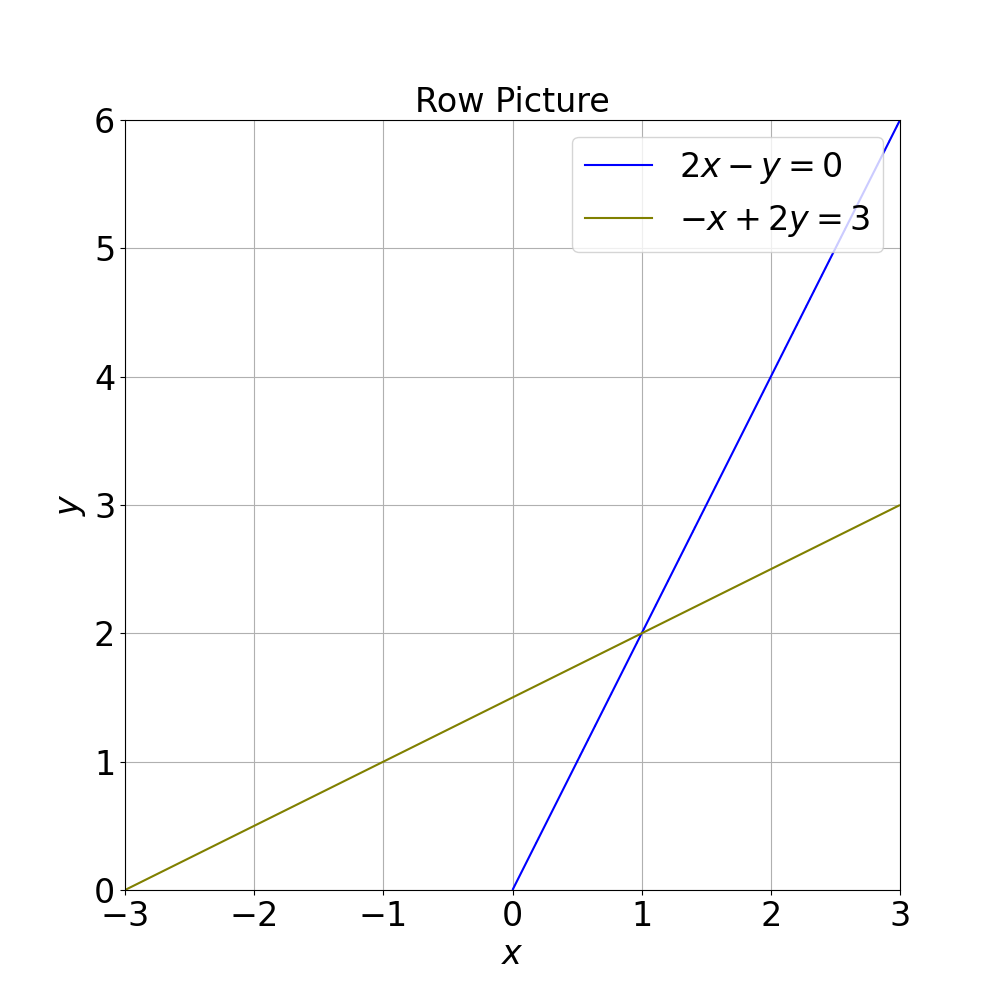
\includegraphics[width=0.7\textwidth]{example equation for the essense of linear algebra.png}
\end{center}

Column picture sees unknowns as scalars of vectors. In (\ref{example equation for the essense of linear algebra}), the system can be written as 
\begin{equation}\label{example equation in form of vectors}
    x\begin{bmatrix}
        2 \\ -1
    \end{bmatrix}+y\begin{bmatrix}
        -1 \\ 2
    \end{bmatrix}=\begin{bmatrix}
        0 \\ 3
    \end{bmatrix}.
\end{equation}
Column picture is relatively difficult to draw on the $xy$-plane; however, one can imagine that, after some stretch (being multiplied by a scalar), the sum of the two vectors, $(2, -1)$ with scalar $x$ and $(-1, 2)$ with scalar $y$, is $(0, 3)$. The true answer for (\ref{example equation for the essense of linear algebra}) is $(x, y)=(1, 2)$. One can easily verify and check that 
\begin{equation*}
    1\cdot\begin{bmatrix}
        2 \\ -1
    \end{bmatrix}+2\cdot\begin{bmatrix}
        -1 \\ 2
    \end{bmatrix}=\begin{bmatrix}
        0 \\ 3
    \end{bmatrix}.
\end{equation*}
Note that the high and thin notation representing a vector in (\ref{example equation in form of vectors}) and the horizontal and with comma notation represent the same thing, i.e., both \begin{equation*}
    \begin{bmatrix}
        2 \\ -1
    \end{bmatrix}
\end{equation*}
and
\begin{equation*}
    (2, -1)
\end{equation*}
represent the vector with first component $2$ and the second component $-1$. They are both called the ``column vector.'' The high and thin notation coincides with the matrix picture, which will be discussed.

In matrix picture, we write the system as
\begin{equation}\label{example equation in form of matrix}
    \begin{bmatrix}
        2 & -1 \\ -1 & 2
    \end{bmatrix}\begin{bmatrix}
        x \\ y
    \end{bmatrix}=\begin{bmatrix}
        0 \\ 3
    \end{bmatrix}.
\end{equation}
In this case, we call $\begin{bmatrix}
    2 & -1 \\ -1 & 2
\end{bmatrix}$ the coefficient matrix and $\begin{bmatrix}
    x \\ y
\end{bmatrix}$ the vector of unknowns. We can simply write \begin{equation*}
    A\bfx=\bfb,
\end{equation*}
where $A$ is the coefficient matrix and $\bfx$ is the vector of unknowns. The benefit of this form is that there might be some beautiful properties for the matrix on the left of the vector $(x, y)$. We are going to discuss those properties in this book.

\subsection{Elimination with Matricies}

\begin{question}
    How to solve the equation \begin{equation*}
        A\bfx=\bfb
    \end{equation*}
    in a systematic way?
\end{question}

We can solve the equation by transforming the matrix $A$ into an upper triangular matrix.

\begin{notation}[Matrix]
    We usuallly use a capital latter to represent a matrix. For example, just as we see, $A$. In addition, we use the lowercase of the letter we just chose and with two numbers $i$ and $j$ to indicate the component $a_{ij}$ on the $i$-th row and the $j$-th column.
\end{notation}

\begin{example}
    Let $$A=\begin{bmatrix}
        4 & 0 \\ -1 & 2
    \end{bmatrix}.$$ Then, $a_{11}=4$, $a_{21}=-1$, $a_{12}=0$, and $a_{22}=2$.
\end{example}

\begin{definition}[Upper Triangular]
    We say a square matrix $A_{n\times n}$ is upper triangular if
    \begin{equation*}
        a_{ij}=0
    \end{equation*}
    for all $n\ge i>j>0$, i.e., \begin{equation*}
        A=\begin{bmatrix}
            & & &\\
           0 & & \ast &\\
           \vdots  & \ddots &  \\
           0 & \cdots & 0 & \ \ 
        \end{bmatrix},
    \end{equation*}
    where the asterisk denotes any possible situation.
\end{definition}

\begin{example}
    Let $$B=\begin{bmatrix}
        4 & -1 \\ 0 & 2
    \end{bmatrix},\quad C=\begin{bmatrix}
        6 & 0 \\ 7 & -13
    \end{bmatrix}.$$ Then, $B$ is upper triangular, and $C$
    is not upper triangular.
\end{example}

If we have an upper triangular coefficient matrix, the solution for the last equation is straightforward. We can then solve the equation above it, followed by the one above that, and so on. To transform a matrix $A$ into an upper triangular matrix $U$, we simply need to multiply $A$ by an appropriate sequence of elementary matrices.

\begin{definition}[Elementary Matrix]
    The effect of elementary matrix is to do row operations. There are three types of elementary matrix: \begin{enumerate}
        \item row switching,
        \item row multiplication, and
        \item row addition.
    \end{enumerate}
    Row switching exchanges two rows, row multiplication makes a specific row being scaled by a non-zero constant, and row addition replace a row with the sum of it and another row with a scalar. Symbolically, we write $$R_i\leftrightarrow R_j$$ to indicate row switching between row $i$ and row $j$, $$kR_i\to R_i$$ to indicate row $i$ is scaled by $k$, and $$R_i+kR_j\to R_i$$ to indicate row $i$ is being added by $R_j$ scaled by $k$.
\end{definition}

Take a matrix $$A=\begin{bmatrix}
    1 & 2 & 1 \\
    3 & 8 & 1 \\
    0 & 4 & 1
\end{bmatrix}$$ for example, we add $-3$ times of the first row to the second row, which makes the matrix $A$ become $$E_{21}A=\begin{bmatrix}
    1 & 2 & 1 \\
    0 & 2 & -2 \\
    0 & 4 & 1
\end{bmatrix}$$ without knowing what $E_{21}$ is now. To make the matrix upper triangular, we add $-2$ times of the second row the the third row, which makes the matrix $A$ become an upper triangular matrix $$U=E_{32}E_{21}A=\begin{bmatrix}
    1 & 2 & 1 \\
    0 & 2 & -2 \\
    0 & 0 & 5
\end{bmatrix}$$
without knowing what $E_{32}$ is now as well.

\subsection{Four Fundamental Subspaces}

\end{document}